%----------------------------------------------------------------------------
\chapter{Writing}\label{app:writing}
%----------------------------------------------------------------------------
\section{Plan before you write: problem to skeleton}\label{app:writing:spine}
Write the argument before the prose. We plan papers in this order, and each step builds on the previous one: problem; context and literature review; gap analysis; research questions; contributions; threat analysis; leading figure; examples; validation plan; spine; figures; skeleton; beats.
\begin{description}
  \item[Problem] The entry point, and the only step you need to start. One paragraph: who has what problem, what goes wrong for them today, and one concrete scenario in which it goes wrong. The scenario becomes the running example, and the paragraph becomes the first page of \tplref{ch:intro}. If you can write it, you can start the literature review; if you cannot, bring what you have to the next consultation and we write it together.
  \item[Spine] One page that fixes the claims, the terminology and the notation of the whole paper. Every chapter, figure and review is checked against it. Its worst enemy is drift: terms, symbols and claims quietly changing between chapters.
  \item[Skeleton mind map] The argument made explicit before any prose: each chapter broken into paragraphs, each paragraph reduced to its topic sentence and a pointer to the evidence that backs it. Drafting then means filling in sentences around a skeleton already known to be sound. A mind map, on paper or in a tool, is the quickest way to draw it; \cref{fig:mindmap} shows one for the guide's running example, a made-up paper, at the level of detail we expect. \Cref{fig:template-skeleton} is the same picture for this template's own beats: the generic argument every chapter file starts from. Your skeleton is built per topic and will not look like either; what carries over is the shape.
  \item[Running example] One concrete scenario that every chapter returns to. Name it once with \texttt{\textbackslash exname} in \texttt{thesis.tex}, introduce it in \tplref{ch:intro}, and revisit it in every chapter in a \texttt{runningexample} box: what each concept, component, measurement or competitor does with it. A reader who follows only the boxes should understand the paper.
  \item[Beats] The moves inside each paragraph of the skeleton: what it establishes, which evidence it uses, what the running example shows there, and how it leads to the next one. \Cref{app:chapters} gives every heading of the template the generic beat of its paragraph. Write your own, specific to your topic, at the top of each paragraph you plan: \texttt{\textbackslash beat\{establishes\}\{evidence\}\{running example\}\{leads to\}}. It prints as a todo, so it disappears from the final version.
\end{description}

\begin{figure}[p]
  \centering
  \begin{forest}
    for tree={
      grow'=0, child anchor=west, parent anchor=east, anchor=west,
      font=\scriptsize, edge={gray!60},
      l sep=6mm, s sep=1.2pt, inner sep=1.5pt,
      edge path={\noexpand\path[\forestoption{edge}](!u.parent anchor) -- +(3mm,0) |- (.child anchor)\forestoption{edge label};},
    },
    where level=0{text width=2.4cm, font=\footnotesize}{},
    where level=1{text width=2.5cm}{},
    where level=2{text width=9.3cm}{},
    [{\textbf{Revoking\\credentials\\with bounded\\staleness}}
      [{\textbf{1 Introduction}}
        [{Digital credentials are checked offline, so a revocation must reach the verifier another way \textit{[incident report, cited]}}]
        [{Running example: a revoked diploma that an employer still accepts, because its status copy is stale}]
        [{REQ1 timely revocation (within $\delta$), REQ2 offline checks, REQ3 holder privacy \textit{[Tab. 6.1]}}]
        [{Gap: no existing approach meets REQ1--REQ3 together \textit{[approaches, cited]}}]
        [{C1 model, C2 registry, C3 evaluation; RQ1 correctness, RQ2 scalability, RQ3 robustness \textit{[Fig. 1.1]}}]
      ]
      [{\textbf{2 Background}}
        [{Issuer, holder, verifier; what a revocation status is and how stale a copy can be \textit{[definition, cited]}}]
        [{Accumulators: membership witness, update cost \textit{[definition, cited]}}]
        [{Permissioned ledgers: writers, readers, finality \textit{[definition, cited]}}]
        [{Dolev--Yao adversary and the Tamarin prover \textit{[tool paper, cited]}}]
      ]
      [{\textbf{3 Approach}}
        [{Overview: a check reads one accumulator witness \textit{[Fig. 3.1]}}]
        [{Model: registry state, revocation, staleness of a verifier's copy \textit{[Def. 3.1]}}]
        [{Check: one witness, offline (REQ2), credential not named (REQ3) \textit{[Alg. 3.1]}}]
        [{Adversary: ADV1 a malicious holder replaying an old status proof, ADV2 a Dolev--Yao network adversary \textit{[ADV1--ADV2]}}]
        [{Assumptions: AS1 sound signatures and accumulator, AS2 clock drift at most $\delta$, AS3 honest-but-curious operator \textit{[AS1--AS3]}}]
        [{Out of scope: denial of service, compromised holder devices}]
        [{Lemma 3.1: status proofs are fresh \textit{[Tamarin model; AS1, AS2]}}]
        [{Theorem 3.1 = SG1: under AS1--AS3, against ADV1 and ADV2, a verifier rejects every credential revoked more than $\delta$ before the check \textit{[Tamarin proof]}}]
        [{Example: the diploma presented with an old status proof is rejected}]
      ]
      [{\textbf{4 Implementation}}
        [{Architecture: registry service, verifier library, reused ledger \textit{[Fig. 3.1]}}]
        [{Design: signed accumulator values, not ledger reads \textit{[alternative rejected]}}]
        [{The verifier's check: signed and younger than $\delta$ \textit{[listing, tests]}}]
        [{Code and scripts archived on Zenodo, with the rerun command \textit{[archived code]}}]
      ]
      [{\textbf{5 Evaluation}}
        [{Setup: one 8-core cloud VM, 10 runs, fresh issuer sets \textit{[rerun command]}}]
        [{RQ1 correctness: proofs per guarantee, tests per requirement \textit{[Tab. 5.1]}}]
        [{The scenario before and after, as a sequence chart \textit{[Fig. 5.1]}}]
        [{RQ2 scalability: checks stay within one round trip up to 10\,000 issuers; a list-based baseline grows linearly \textit{[Fig. 5.2]}}]
        [{Storage grows with the credentials ever issued \textit{[Fig. 5.2]}}]
        [{RQ3 robustness: a ledger node crash, a revocation burst, clock drift and $\delta$ varied \textit{[Tab. 5.2, Fig. 5.3]}}]
        [{Threats to validity: synthetic issuer sets, one cloud VM}]
      ]
      [{\textbf{6 Related work}}
        [{Family A: how it works, which of REQ1--REQ3 it gives up \textit{[approaches, cited]}}]
        [{Family B: how it works, which of REQ1--REQ3 it gives up \textit{[approaches, cited]}}]
        [{Family C: how it works, which of REQ1--REQ3 it gives up \textit{[approaches, cited]}}]
        [{Gap matrix: no family meets REQ1--REQ3 together \textit{[Tab. 6.1, Fig. 6.1]}}]
      ]
      [{\textbf{7 Conclusion}}
        [{C1--C3 restated with their evidence \textit{[Thm 3.1, Fig. 5.2, Tab. 5.1]}}]
        [{LIM1 synthetic workloads \textit{[threats to validity]}}]
        [{LIM2 the registry cannot force an issuer to revoke \textit{[scope of SG1]}}]
        [{Future work: real issuer workloads; holding issuers to their revocation duty}]
      ]
    ]
  \end{forest}
  \caption{A skeleton mind map for the guide's running example, the credential revocation registry, whose items \cref{app:chapters} renders chapter by chapter, so one paper can be followed from skeleton to items. Every leaf is one paragraph's topic sentence, and the bracketed italics name the evidence behind it: a theorem, a model, a table, a figure or a citation. A skeleton at this level of detail shows whether the argument holds before a sentence of prose exists, and it is what the spine anchor of \cref{tab:lifecycle} is checked against. Copy the shape, not the topic: one leaf per paragraph, evidence on every leaf that makes a claim, and the running example visible in every chapter.}\label{fig:mindmap}
\end{figure}


\begin{figure}[p]
  \centering
  \begin{forest}
    for tree={
      grow'=0, child anchor=west, parent anchor=east, anchor=west,
      font=\scriptsize, edge={gray!60},
      l sep=6mm, s sep=1.2pt, inner sep=1.5pt,
      edge path={\noexpand\path[\forestoption{edge}](!u.parent anchor) -- +(3mm,0) |- (.child anchor)\forestoption{edge label};},
    },
    where level=0{text width=2.4cm, font=\footnotesize}{},
    where level=1{text width=2.5cm}{},
    where level=2{text width=9.3cm}{},
    [{\textbf{The template's beats}}
      [{\textbf{1 Introduction}}
        [{Context: why the field matters now \textit{[a trend, a regulation or an incident, cited]}}]
        [{Problem: the concrete problem, ending in a one-sentence statement \textit{[the running example]}}]
        [{Requirements: what a solution must do \textit{[one requirement per failure of the example; the rows of the gap matrix]}}]
        [{Gap: no existing approach meets them together \textit{[the closest approaches, cited]}}]
        [{Contributions: what this work claims, as checkable items \textit{[the chapters behind each]}}]
      ]
      [{\textbf{2 Background}}
        [{The first concept the approach relies on; notation defined once \textit{[a definition and a citation]}}]
        [{The second concept \textit{[a definition and a citation]}}]
      ]
      [{\textbf{3 Approach}}
        [{Overview: how it works end to end \textit{[the architecture figure]}}]
        [{The formal model or the design decisions \textit{[each decision with the alternative rejected]}}]
        [{Threat model: the adversary's capabilities, who is trusted, the cryptographic assumptions, what is out of scope, and the guarantees \textit{[a proof, a mechanised proof or a measurement per guarantee]}}]
      ]
      [{\textbf{4 Implementation}}
        [{What was built and how it realises the approach \textit{[components mapped to code; the archived artifact]}}]
        [{Design decisions and the problems a straightforward build runs into \textit{[each with the alternative rejected]}}]
        [{The part that did not exist before \textit{[the key listing and the tests that cover it]}}]
      ]
      [{\textbf{5 Evaluation}}
        [{Setup: how the measurements were made \textit{[hardware, versions, workloads, repetitions, the rerun command]}}]
        [{Correctness on the example and on every requirement case \textit{[test, proof or model-checking results]}}]
        [{How the cost grows with the input \textit{[the scalability figure]}}]
        [{Behaviour when the assumptions are stressed \textit{[the robustness table, with each perturbation's setup]}}]
        [{Threats to validity and what was done about each \textit{[the mitigations]}}]
      ]
      [{\textbf{6 Related work}}
        [{How each family of approaches works and where it falls short \textit{[citations, the positioning figure and the gap matrix]}}]
        [{The gap in one sentence, closed by this work \textit{[the gap matrix and the evaluation results]}}]
      ]
      [{\textbf{7 Conclusion}}
        [{Each contribution and its evidence \textit{[the chapters behind C1--C3]}}]
        [{What is still open, and the next step for each limitation \textit{[the threats to validity]}}]
      ]
    ]
  \end{forest}
  \caption{The template's own beats drawn as a skeleton: one leaf per beat of \cref{app:chapters}, the topic it establishes first and its evidence in brackets. This is the generic argument the template starts you from, not a skeleton to copy: \cref{fig:mindmap} shows what a topic's own skeleton looks like once the claims, examples and evidence are specific, and yours will have more leaves where your contribution is and fewer elsewhere.}\label{fig:template-skeleton}
\end{figure}

\section{The essentials}\label{app:writing:essentials}
Every paper of this kind contains the same two dozen elements, whatever its topic: a problem statement, requirements, a leading figure, a threat model, research questions, a gap matrix, a summary with its evidence, and the rest of the list below. They are the leaves of \cref{fig:template-skeleton} that a reviewer looks for by name, and the review sheet scores each of them somewhere; the letter after each row names the criterion. The lint calls them the \emph{essentials} and measures every paper against the same list, so the Checks page at the front of the draft shows where yours stands, and the job summary of your repository's CI opens with the same marks in one line. The list lives in \texttt{scripts/lint/essentials.lua}, and this section is printed from it by \texttt{make essentials}: delete the template's skeleton chapters and the list still holds. Each row links to the same item in action in \cref{app:chapters}.

% generated by texlua scripts/lint.lua essentials --guide (make essentials); do not edit
\definecolor{lintaccent}{RGB}{155,28,28}\definecolor{lintmute}{gray}{0.38}
\providecommand{\lintdisc}[3]{\tikz[baseline=-.6ex]{\draw[#2,line width=.45pt,fill=white] (0,0) circle (#1);\ifcase#3\relax\or\fill[#2] (0,0) -- (0,#1) arc[start angle=90,end angle=0,radius=#1] -- cycle;\or\fill[#2] (0,0) -- (0,#1) arc[start angle=90,end angle=-90,radius=#1] -- cycle;\or\fill[#2] (0,0) -- (0,#1) arc[start angle=90,end angle=-180,radius=#1] -- cycle;\or\fill[#2] (0,0) circle (#1);\fi}}
\providecommand{\lintball}[2][black]{\lintdisc{.62ex}{#1}{#2}}
\providecommand{\lintbigball}[2][black]{\lintdisc{.8ex}{#1}{#2}}
The lint places each essential on a ladder of five levels: \lintball{0} missing; \lintball{1} a placeholder, only TODO or the template's own text; \lintball{2} started, your own text but not enough of it; \lintball{3} written; \lintball{4} used where the argument needs it. An essential with no condition for its use is \lintball{4} once written. The phase in \texttt{thesis.tex} asks every essential for a level: \textsc{plan} \lintball{1}, \textsc{draft} \lintball{2}, \textsc{polish} and \textsc{final} \lintball{4}. An essential is found by its label first, then by a heading that contains one of the words given. Text is your own when it is neither a TODO line nor a line of the template, and floats, tagged lists and example boxes count toward their own essentials, not toward the text around them.

{\small\begin{xltabular}{\linewidth}{@{}>{\raggedright\arraybackslash}p{.25\linewidth}>{\raggedright\arraybackslash}X>{\raggedright\arraybackslash}p{.3\linewidth}@{}}
\toprule \textbf{Essential} & \textbf{What it is, and why} & \textbf{Written, and used} \\ \midrule \endfirsthead
\toprule \textbf{Essential} & \textbf{What it is, and why} & \textbf{Written, and used} \\ \midrule \endhead \bottomrule \endlastfoot
\multicolumn{3}{@{}l}{\textsc{Front matter}} \\
\textbf{Abstract and Kivonat}\newline{\footnotesize\color{lintmute}\texttt{\textbackslash chapter*\{Kivonat\}} and \texttt{\{Abstract\}}}\newline{\footnotesize In action: \cref{app:writing:abstract}} & The paper in one paragraph, in English and in Hungarian; the reviewer reads it first and the registration carries it.\hfill{\footnotesize\color{lintmute}(E)} & 100 own words in each.\newline Written is enough. \\
\addlinespace[.8ex]\multicolumn{3}{@{}l}{\textsc{Introduction}} \\
\textbf{Context}\newline{\footnotesize\color{lintmute}\texttt{par:context}, or a heading with \emph{context} or \emph{motivation}}\newline{\footnotesize In action: \cref{app:chapters:context}} & Why the topic matters now: a trend, a regulation or an incident, cited; relevance is scored in C.\hfill{\footnotesize\color{lintmute}(C, E)} & 40 own words.\newline Written is enough. \\
\textbf{Problem statement}\newline{\footnotesize\color{lintmute}\texttt{par:problem}, or a heading with \emph{problem}}\newline{\footnotesize In action: \cref{app:chapters:problem}} & The concrete problem, ending in a one-sentence statement; the sheet's E names the problem statement as a must.\hfill{\footnotesize\color{lintmute}(E)} & 40 own words.\newline Written is enough. \\
\textbf{Running example}\newline{\footnotesize\color{lintmute}\texttt{\textbackslash exname} and the example box}\newline{\footnotesize In action: \cref{app:chapters:problem}} & One small scenario, named once in thesis.tex (\textbackslash{}exname) and revisited in a box in every chapter, so the reader can follow each step.\hfill{\footnotesize\color{lintmute}(A)} & Named, and the introduction's box in your own words.\newline Used when an example box in every main chapter. \\
\textbf{Requirements}\newline{\footnotesize\color{lintmute}items labelled \texttt{req:}}\newline{\footnotesize In action: \cref{app:chapters:requirements}} & What a solution must do, one checkable item each; they are the rows of the gap matrix and the yardstick of the evaluation.\hfill{\footnotesize\color{lintmute}(D/1)} & Every item in your own words.\newline Used when each requirement is referenced in the related work and in the evaluation, and each derived requirement (dr:) in the evaluation. \\
\textbf{Gap, in brief}\newline{\footnotesize\color{lintmute}\texttt{par:gap}, or a heading with \emph{gap}}\newline{\footnotesize In action: \cref{app:chapters:introgap}} & That no existing approach meets the requirements together; the novelty claim, made before the full comparison.\hfill{\footnotesize\color{lintmute}(D/1)} & 40 own words.\newline Used when it points to the full comparison: the related-work chapter, the gap matrix or the positioning figure. \\
\textbf{Leading figure}\newline{\footnotesize\color{lintmute}\texttt{fig:overview}}\newline{\footnotesize In action: \cref{fig:guide:overview}} & The problem, the contributions and the headline result in one picture; the reviewer looks here first.\hfill{\footnotesize\color{lintmute}(B/1)} & Your own content, and a caption of at least a sentence.\newline Used when it is referenced from the text. \\
\textbf{Contributions}\newline{\footnotesize\color{lintmute}items labelled \texttt{c:}}\newline{\footnotesize In action: \cref{app:chapters:contributions}} & What this work claims, as checkable items; the sheet's E names stating the main contribution as a must.\hfill{\footnotesize\color{lintmute}(E)} & Every item in your own words.\newline Used when each contribution points to the chapter that delivers it and is referenced in the conclusion. \\
\addlinespace[.8ex]\multicolumn{3}{@{}l}{\textsc{Approach}} \\
\textbf{Architecture figure}\newline{\footnotesize\color{lintmute}\texttt{fig:architecture}}\newline{\footnotesize In action: \cref{fig:guide:architecture}} & The approach end to end, with what is yours set apart from what is reused.\hfill{\footnotesize\color{lintmute}(B/1)} & Your own content, and a caption of at least a sentence.\newline Used when it is referenced from the text. \\
\textbf{Threats}\newline{\footnotesize\color{lintmute}items labelled \texttt{thr:}}\newline{\footnotesize In action: \cref{app:chapters:adversary}} & Who the adversary is and what it can do; a reviewer of a security topic looks for it first.\hfill{\footnotesize\color{lintmute}(D/2)} & Every item in your own words.\newline Used when each threat is referenced in the approach, where a guarantee or an assumption meets it. \\
\textbf{Assumptions}\newline{\footnotesize\color{lintmute}items labelled \texttt{asm:}}\newline{\footnotesize In action: \cref{app:chapters:assumptions}} & Who is trusted and which properties the guarantees rest on, stated so a reviewer can check them.\hfill{\footnotesize\color{lintmute}(D/2)} & Every item in your own words.\newline Used when each assumption is referenced in the approach, by a guarantee or a proof. \\
\textbf{Guarantees}\newline{\footnotesize\color{lintmute}items labelled \texttt{g:}}\newline{\footnotesize In action: \cref{app:chapters:guarantees}} & What the approach guarantees under the assumptions, against the threats; each is what the evaluation checks.\hfill{\footnotesize\color{lintmute}(D/2)} & Every item in your own words.\newline Used when each guarantee is referenced in the evaluation, as a row of the correctness table. \\
\addlinespace[.8ex]\multicolumn{3}{@{}l}{\textsc{Evaluation}} \\
\textbf{Research questions}\newline{\footnotesize\color{lintmute}items labelled \texttt{rq:}}\newline{\footnotesize In action: \cref{app:chapters:research-questions}} & The questions the evaluation answers: correctness, scale and robustness at least.\hfill{\footnotesize\color{lintmute}(E)} & Every item in your own words.\newline Used when each research question is referenced in the evaluation, where it is answered. \\
\textbf{Setup and artifact}\newline{\footnotesize\color{lintmute}\texttt{sec:setup}, or a heading with \emph{setup}}\newline{\footnotesize In action: \cref{app:chapters:setup}} & How the measurements were made, so each can be checked, and where the archived artifact is.\hfill{\footnotesize\color{lintmute}(D/2)} & 100 own words.\newline Used when the evaluation cites the archived artifact with a real DOI. \\
\textbf{Correctness}\newline{\footnotesize\color{lintmute}\texttt{tab:correctness}}\newline{\footnotesize In action: \cref{tab:guide:correctness}} & How each guarantee and requirement was checked: proved, tested or model-checked, with the result.\hfill{\footnotesize\color{lintmute}(D/2)} & Your own content, and a caption of at least a sentence.\newline Used when it is referenced from the text, and every guarantee (g:) has a row in it. \\
\textbf{Scalability}\newline{\footnotesize\color{lintmute}\texttt{sec:scalability}, or a heading with \emph{scalab} or \emph{scaling} or \emph{performance}}\newline{\footnotesize In action: \cref{app:chapters:scalability}} & How the cost grows with the input; the review sheet scores the evaluation's depth in E.\hfill{\footnotesize\color{lintmute}(E)} & 100 own words.\newline Used when the section holds a figure or table that the text references. \\
\textbf{Robustness}\newline{\footnotesize\color{lintmute}\texttt{sec:robustness}, or a heading with \emph{robust}}\newline{\footnotesize In action: \cref{app:chapters:robustness}} & How the system behaves when its assumptions are stressed; scored apart from scalability.\hfill{\footnotesize\color{lintmute}(E)} & 100 own words.\newline Used when the section holds a figure or table that the text references. \\
\textbf{Threats to validity}\newline{\footnotesize\color{lintmute}\texttt{sec:validity}, or a heading with \emph{validity}}\newline{\footnotesize In action: \cref{app:chapters:validity}} & What could make the results wrong or not generalise, and what was done about each.\hfill{\footnotesize\color{lintmute}(D/2)} & 100 own words.\newline Written is enough. \\
\addlinespace[.8ex]\multicolumn{3}{@{}l}{\textsc{Related work}} \\
\textbf{Positioning figure}\newline{\footnotesize\color{lintmute}\texttt{fig:positioning}}\newline{\footnotesize In action: \cref{fig:guide:positioning}} & The related work on the two properties that separate it most, with this work in the cell no one else reaches.\hfill{\footnotesize\color{lintmute}(B/2)} & Your own content, and a caption of at least a sentence.\newline Used when it is referenced from the text. \\
\textbf{Gap matrix}\newline{\footnotesize\color{lintmute}\texttt{tab:related}}\newline{\footnotesize In action: \cref{tab:guide:related}} & Each requirement against the closest approaches: every other approach misses something, this work meets all.\hfill{\footnotesize\color{lintmute}(D/1)} & Your own content, and a caption of at least a sentence.\newline Used when rows are the requirements, this work's column is all met with pointers to results, and every other approach misses one. \\
\textbf{The gap}\newline{\footnotesize\color{lintmute}\texttt{sec:gap}, or a heading with \emph{gap}}\newline{\footnotesize In action: \cref{app:chapters:gap}} & The gap in one sentence, shown closed by this work's results.\hfill{\footnotesize\color{lintmute}(D/1)} & 100 own words.\newline Used when it is based on the gap matrix (references tab:related). \\
\addlinespace[.8ex]\multicolumn{3}{@{}l}{\textsc{Conclusion}} \\
\textbf{Summary with evidence}\newline{\footnotesize\color{lintmute}\texttt{sec:summary}, or a heading with \emph{summary}}\newline{\footnotesize In action: \cref{app:chapters:summary}} & Each contribution restated with the result behind it; the reviewer checks here that the promises were kept.\hfill{\footnotesize\color{lintmute}(E)} & 100 own words.\newline Used when it cites an evaluation result: the evaluation chapter, a research question, a figure, a table or a theorem. \\
\textbf{Limitations}\newline{\footnotesize\color{lintmute}items labelled \texttt{lim:}}\newline{\footnotesize In action: \cref{app:chapters:future}} & What this work does not do, stated before a reviewer finds it.\hfill{\footnotesize\color{lintmute}(E)} & Every item in your own words.\newline Written is enough. \\
\textbf{Future work}\newline{\footnotesize\color{lintmute}\texttt{sec:future}, or a heading with \emph{future}}\newline{\footnotesize In action: \cref{app:chapters:future}} & What is still open, and the next step that would lift each limitation.\hfill{\footnotesize\color{lintmute}(E)} & 100 own words.\newline Written is enough. \\
\end{xltabular}}


\section{The leading figure (vezérábra)}\label{app:writing:figure}
The leading figure (\tplref{fig:overview}) explains the central idea in one picture: the problem, the contributions, and the result. Decide what a reader should take away from it, draw that, and write the caption so that the figure stands without the text. Make what is yours visible at a glance. The template's figures use one colour for everything that is yours, blue, through the \texttt{ours} TikZ style; the problem is red, the result green, and reused or external parts are grey (\texttt{prior}). Every work has at least two components, and all of them get the same blue, so the reader sees the extent of your contribution in one look; the caption says which colour is which. A reviewer who cannot tell your contribution from the surrounding system in the first figure will assume the smaller part is yours. Draft it early, in the research phase, and treat it as exploratory until the spine is agreed: many papers find their argument while drawing it. \Cref{fig:collage} shows the leading figures of four papers from our group.

\begin{figure}[!ht]
  \centering
  \begin{subfigure}[t]{0.48\linewidth}
    \centering
    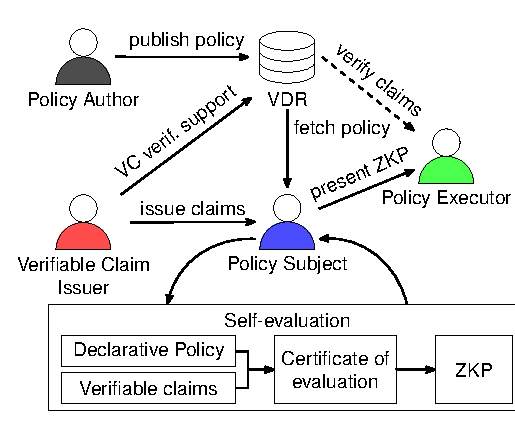
\includegraphics[width=\linewidth,height=5.2cm,keepaspectratio]{guide/figures/collage/eurocybersec2024}
    \caption{A policy is evaluated by its own subject and proven in zero knowledge: the actors and the flows between them, nothing else.}\label{fig:collage:ecs}
  \end{subfigure}\hfill
  \begin{subfigure}[t]{0.48\linewidth}
    \centering
    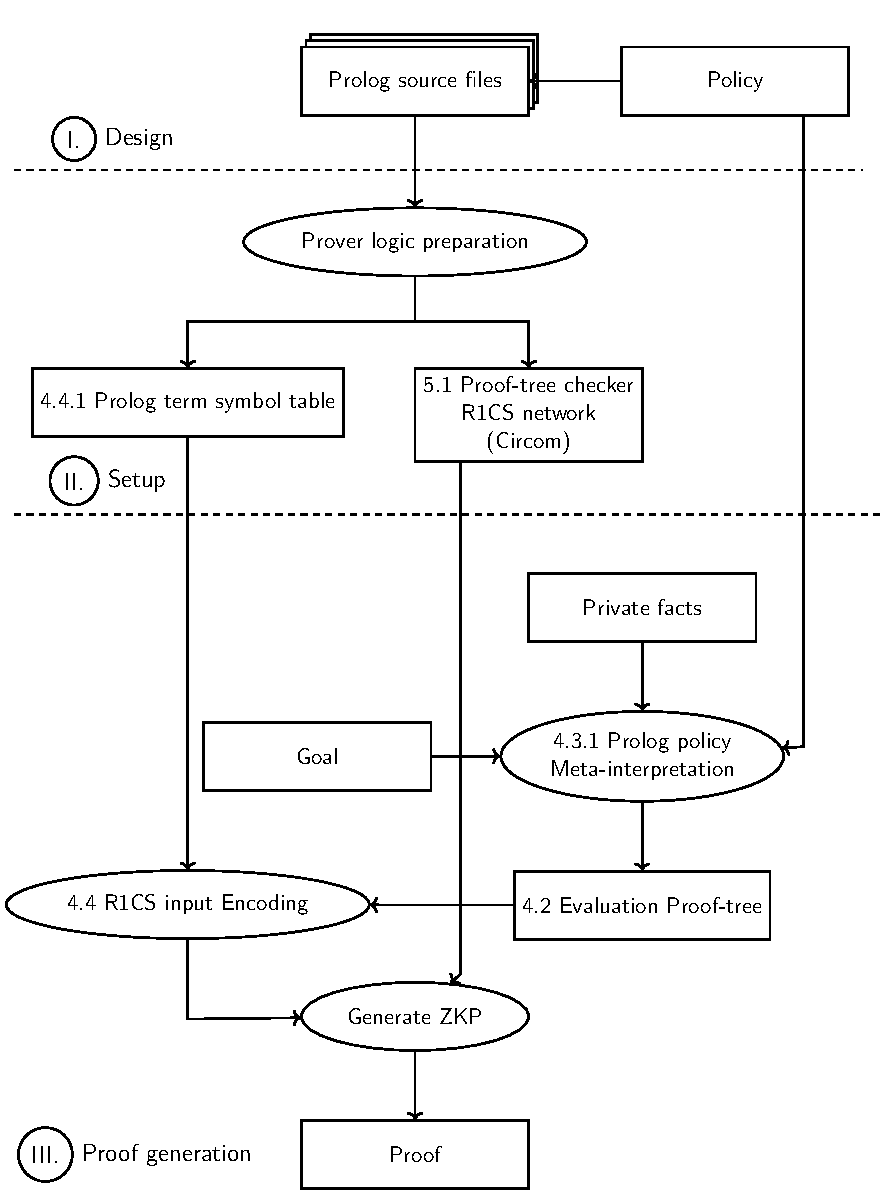
\includegraphics[width=\linewidth,height=5.2cm,keepaspectratio]{guide/figures/collage/tdk2023}
    \caption{The toolchain of the same idea as a TDK paper: every stage from policy to proof, so the reader sees where the contribution sits.}\label{fig:collage:tdk}
  \end{subfigure}

  \medskip
  \begin{subfigure}[t]{0.48\linewidth}
    \centering
    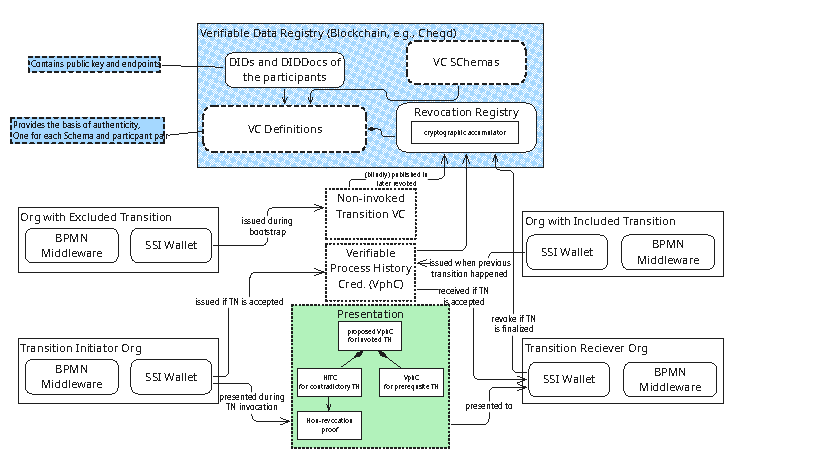
\includegraphics[width=\linewidth,height=5.2cm,keepaspectratio]{guide/figures/collage/bpm2025}
    \caption{Self-orchestrated business collaborations: the architecture with the data model folded in, one picture for both.}\label{fig:collage:bpm25}
  \end{subfigure}\hfill
  \begin{subfigure}[t]{0.48\linewidth}
    \centering
    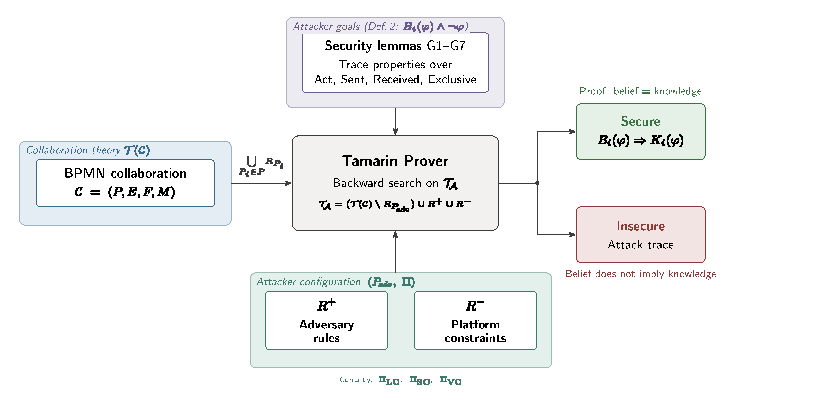
\includegraphics[width=\linewidth,height=5.2cm,keepaspectratio]{guide/figures/collage/bpm2026}
    \caption{From a BPMN collaboration to a security analysis: inputs on the left, the method in the middle, the verdicts on the right.}\label{fig:collage:bpm26}
  \end{subfigure}
  \caption{Leading figures of four papers from the group: (a) the EuroCyberSec 2024 workshop paper on self-evaluated policies~\cite{guide:farkas2024selfevaluated}, (b) the 2023 TDK paper it grew out of~\cite{guide:farkas2023tdk}, (c) the self-orchestration model for business collaborations~\cite{guide:farkas2025selforchestration}, and (d) the formal security analysis of BPMN collaborations~\cite{guide:farkas2026trustnopool}. Each one shows the problem, the contribution and the result in a single picture, and each was drawn before the paper was written.}\label{fig:collage}
\end{figure}

When the contribution is spread over several chapters, \cref{app:writing:depgraph} draws the whole paper instead.

\section{An alternative: the paper as a dependency graph}\label{app:writing:depgraph}
The skeleton mind map (\cref{fig:mindmap}) is a tree of chapters and their paragraphs. Draw an arrow from each paragraph to every paragraph that needs it, and the tree becomes a dependency graph of the paper (\cref{fig:depgraph}). Lay it out in bands, one per chapter in reading order, with each band's paragraphs in their order in the chapter. Colour green the paragraphs that deliver a contribution, tag each with its contribution, and leave the rest white. The green is for the reviewer: before reading a sentence, they see where your contribution is, how much of the paper it fills, what it stands on, and which evaluation question tests it. Green marks paragraphs here, not components, so the architecture figure keeps the blue of \texttt{ours} for the parts of the system you built.

\begin{figure}[!ht]
  \centering
  \begin{tikzpicture}[
      x=25mm, y=-17mm,
      para/.style={draw=gray!60, fill=white, rounded corners=1pt, text width=20mm, minimum height=10mm,
        align=center, font=\footnotesize, inner sep=2pt, execute at begin node={\hyphenpenalty=10000}},
      contrib/.style={para, draw=green!50!black, line width=1.1pt, fill=green!15},
      dep/.style={-Stealth, gray!70, semithick}]
    % One band per chapter, in reading order; within a band, paragraphs keep their order in the chapter.
    \begin{scope}[on background layer]
      \foreach \r/\chap in {0/Introduction, 1/Background, 2/Approach, 3/Implementation,
                            4/Evaluation, 5/Related work, 6/Conclusion} {
        \pgfmathsetmacro{\n}{int(\r+1)}
        \pgfmathparse{mod(\r,2) ? "white" : "gray!8"}
        \fill[\pgfmathresult] (-1.6,\r-0.47) rectangle (5.5,\r+0.47);
        \node[anchor=west, font=\footnotesize] at (-1.58,\r) {\textbf{\n}~\chap};
      }
    \end{scope}
    \node[para]    (problem)  at (0,0) {Problem: a stale status};
    \node[para]    (req)      at (1,0) {REQ1--REQ3};
    \node[para]    (gap)      at (2,0) {Gap: none meets all three};
    \node[para]    (claims)   at (3,0) {Contributions C1--C3};
    \node[para]    (cred)     at (0,1) {Revocation status};
    \node[para]    (acc)      at (1,1) {Accumulators};
    \node[para]    (ledger)   at (2,1) {Permissioned ledgers};
    \node[para]    (dy)       at (3,1) {Dolev--Yao and Tamarin};
    \node[contrib] (model)    at (0,2) {\textbf{C1} Registry model};
    \node[contrib] (check)    at (1,2) {\textbf{C1} Check with one witness};
    \node[para]    (threat)   at (3,2) {Adversary and assumptions};
    \node[contrib] (thm)      at (4,2) {\textbf{C1} Theorem: SG1};
    \node[contrib] (arch)     at (0,3) {\textbf{C2} Architecture};
    \node[contrib] (design)   at (1,3) {\textbf{C2} Signed values};
    \node[contrib] (code)     at (2,3) {\textbf{C2} The check, tested};
    \node[contrib] (rq1)      at (2,4) {\textbf{C3} RQ1 correctness};
    \node[contrib] (rq2)      at (3,4) {\textbf{C3} RQ2 scalability};
    \node[contrib] (rq3)      at (4,4) {\textbf{C3} RQ3 robustness};
    \node[para]    (validity) at (5,4) {Threats to validity};
    \node[para]    (families) at (0,5) {Families A--C};
    \node[para]    (matrix)   at (1,5) {Gap matrix};
    \node[para]    (summary)  at (3,6) {Summary of C1--C3};
    \node[para]    (limits)   at (4,6) {Limitations};
    \node[para]    (future)   at (5,6) {Future work};
    % An arrow points from a paragraph to the paragraph that needs it.
    \draw[dep] (problem) -- (req);
    \draw[dep] (req) -- (gap);
    \draw[dep] (gap) -- (claims);
    \draw[dep] (cred) -- (model);
    \draw[dep] (acc) -- (check);
    \draw[dep] (model) -- (check);
    \draw[dep] (dy) -- (threat);
    \draw[dep] (threat) -- (thm);
    \draw[dep] (check.south east) .. controls (2.1,2.62) and (3.3,2.62) .. (thm.south west);
    \draw[dep] (check) -- (arch);
    \draw[dep] (ledger) -- (design.north east);
    \draw[dep] (arch) -- (design);
    \draw[dep] (design) -- (code);
    \draw[dep] (thm.250) -- (rq1.north east);
    \draw[dep] (code) -- (rq1);
    \draw[dep] (code.east) -| ($(rq2.north)+(-0.2,0)$);
    \draw[dep] (thm) -- (rq3);
    \draw[dep] (families) -- (matrix);
    \draw[dep] (rq1) -- (summary);
    \draw[dep] (rq2) -- (summary);
    \draw[dep] (rq3) -- (summary);
    \draw[dep] (validity) -- (limits);
    \draw[dep] (limits) -- (future);
  \end{tikzpicture}
  \caption{The guide's running example as a dependency graph: each contribution stands on the background and leads to an evaluation question. One band per chapter in reading order, one box per paragraph in its order within the chapter, and an arrow from a paragraph to each paragraph that needs it. Green boxes deliver the contribution in their tag, white boxes are context, and every arrow runs to a later chapter or rightwards within one. It is the paper of \cref{fig:mindmap} with fewer boxes: the figure keeps the paragraphs that carry the argument, not all of them.}\label{fig:depgraph}
\end{figure}

It can take either of two places in the paper. As \tplref{fig:overview}, it suits a work whose contribution is a model, a tool and an evaluation spread over several chapters, which a problem-to-result picture would flatten into one box; the green has to read at a glance, so merge a chapter's paragraphs into its sections when there are many. As the figure of the structure paragraph at the end of the introduction (\cref{app:chapters:structure}), it replaces the list of chapters: the paragraph says what the bands, arrows and colours mean, and the figure shows the rest.

Drawing it also checks the skeleton before any prose exists. Every arrow should run down to a later chapter or right within one; an arrow pointing up or left is a paragraph that needs something the reader has not reached yet, so move one of the two, or say where the missing part comes. A green box with no path to an evaluation question is a contribution the paper claims but does not back. A background box that no arrow leaves is background the paper does not use. Draw only the arrows a reader needs to follow the argument: the figure shows where the contribution is, not every cross-reference.

\section{Figures}\label{app:writing:figures}
Every figure is vector. Draw the final version in TikZ, in the paper repository, so that it uses the paper's fonts, scales without loss, and can be fixed by anyone in the last week; \cref{app:latex} shows the TikZ and pgfplots setup of this template. Sketch in \href{https://www.drawio.com/}{draw.io} while the figure is still changing, then redraw it in TikZ once the spine is agreed. An exported PDF is the last resort, for a figure from another paper or a screenshot. Plots come from pgfplots reading the CSV that \texttt{just reproduce} writes, so a changed measurement changes the figure without anyone redrawing it. Every axis has a label with a unit, and nothing in a figure is smaller than 10\,pt in print.

\section{Captions}\label{app:writing:captions}
A caption is the figure's own paragraph, and a reader who reads only figures and captions should follow the paper. A caption explains the figure; it does not describe it. Its first sentence states what the figure shows as a claim. Then it puts that claim in context: which question it answers, what a reader needs to know to understand it, and why the result is what it is. Anything the reader could get from the axes and the legend does not belong in the caption; anything they could not, does: the concept being measured, the assumption behind the setup, the reason one curve bends. A diagram gets two or three sentences; a result figure gets as many as the explanation needs. Nature's captions are the model, for example those of \citet{guide:gulyas2015navigable}; \cref{fig:caption-example} is one in this template's style.

\begin{figure}[!ht]
  \centering
  \begin{tikzpicture}
    \begin{groupplot}[group style={group size=2 by 1, horizontal sep=1.6cm}, width=0.5\linewidth, height=5cm,
      xmode=log, log basis x=10, xlabel={Issuers in the registry}, grid=major, tick label style={font=\scriptsize}, label style={font=\footnotesize}, legend style={font=\scriptsize, at={(0.03,0.97)}, anchor=north west}]
      \nextgroupplot[ylabel={Median check latency [ms]}, ymode=log, title={(a)}, title style={font=\footnotesize}]
        \addplot+[mark=*, blue!70!black] coordinates {(10,31) (100,33) (1000,35) (10000,38)};
        \addplot+[mark=square*, gray] coordinates {(10,34) (100,61) (1000,310) (10000,2900)};
        \addplot[dashed, red!70!black] coordinates {(10,40) (10000,40)};
        \legend{this work, list-based baseline, one round trip}
      \nextgroupplot[ylabel={Registry size [MB]}, title={(b)}, title style={font=\footnotesize}, ymode=log]
        \addplot+[mark=*, blue!70!black] coordinates {(10,2) (100,12) (1000,110) (10000,1050)};
        \addplot+[mark=square*, gray] coordinates {(10,1) (100,3) (1000,21) (10000,190)};
    \end{groupplot}
  \end{tikzpicture}
  \caption{\textbf{Revocation checks stay within one network round trip up to 10\,000 issuers, while the list-based baseline grows linearly.} This is the scalability question, RQ2: a registry that serves a national ecosystem must answer a check without the verifier noticing. Our registry stays flat because a check reads one accumulator witness whatever the number of issuers, whereas the baseline scans the issuer's list. The price is the storage in panel (b), which grows with the number of credentials ever issued; the robustness analysis shows this stays under what a single server holds today. Medians over 10 runs with fresh issuer sets, on one 8-core VM in the BME cloud. (Illustrative numbers for the guide's running example.)}\label{fig:caption-example}
\end{figure}

\section{The abstract}\label{app:writing:abstract}
The abstract has a job before it has a structure: it must convince two readers that the paper is worth their time. The first is us, when you register the summary on the portal; the second is the committee that assigns the reviewers and, later, the reviewers themselves, who read it before anything else. Both have to come away believing that the topic is \textbf{relevant}, that solving it is \textbf{non-trivial}, that what you did is \textbf{novel}, and that it is \textbf{correct}: the same four things the review sheet scores (\cref{app:tdk:sheet}). Then follow \weblink{https://www.nature.com/documents/nature-summary-paragraph.pdf}{Nature's summary paragraph guide}; the abstract in this template already has its seven steps as placeholders.

\section{Style}
\begin{itemize}
  \item The Chicago School of Writing lectures: \href{https://www.youtube.com/watch?v=vtIzMaLkCaM}{part I}, \href{https://www.youtube.com/watch?v=aFwVf5a3pZM}{part II}, \href{https://www.youtube.com/watch?v=gphdfSwYMWU}{part III}.
  \item \href{https://www.youtube.com/watch?v=Unzc731iCUY}{MIT: How to Speak}, for the conference talk.
  \item Good examples: Leslie Lamport's papers, the Raft paper, and the figures and captions of \citet{guide:gulyas2015navigable}.
  \item For contrast, read the original Paxos and PBFT papers next to the Raft paper: all three carry great ideas, and the Raft paper was written so that its idea is the easy part.
\end{itemize}

\section{Disclose AI use}\label{app:writing:ai}
The faculty's \href{https://vik.bme.hu/page/1346/}{guidelines on the use of AI} set these rules, and this template follows them:
\begin{itemize}
  \item \textbf{Declare every use} in the faculty's declaration (\tplref{aidecl}, after the bibliography): which tool, for what, which parts of the paper, and how large a share. It is required for every thesis and cannot be waived; we require it for the TDK too.
  \item \textbf{Cite facts and conclusions from an AI answer} that were not in your prompt, like any other source, in the faculty's required MLA form: a one-sentence summary of the prompt, the model with its version, the company, the date, and a link to the conversation if possible. The faculty's example: \enquote{Examples of harm-reduction initiatives} prompt. ChatGPT-4o, OpenAI, February 10, 2025. \texttt{bib/references.bib} has a commented entry in this form.
\end{itemize}
\begin{itemize}
  \item \textbf{Keep the essential work your own.} The supervisor decides whether enough of the results are clearly yours, and a submission is not approved if AI use is disproportionately large or touches the essential parts. In the faculty's words: \enquote{If the task was to develop software and most of it was produced with generative AI, this is not acceptable}, while AI-supported software that serves your own algorithm, procedure or analysis is acceptable.
\end{itemize}
Verifying an AI answer is always your responsibility; an answer can never be a reference by itself. \Cref{app:code:ai} covers the tools.
